%!TEX program = xelatex
% 完整编译: xelatex -> bibtex -> xelatex -> xelatex
\documentclass[lang=cn,11pt,a4paper,cite=numbers]{elegantpaper}
\usepackage{xfp}
\usepackage{tikz}

\title{如何理解傅里叶变换公式?}
\author{郑晖}
% \institute{}

% \version{0.09}
\date{\zhtoday}

% 本文档命令
\usepackage{array}
\newcommand{\ccr}[1]{\makecell{{\color{#1}\rule{1cm}{1cm}}}}

\begin{document}

\maketitle

\begin{abstract}
傅里叶变换的核心是从时域到频域的变换,而这种变换是通过一组特殊的正交基来实现的。
\keywords{傅里叶变换}
\end{abstract}

\section{时域}
  时域是描述一个数学函数或物理信号对时间的关系,这也是我们日常生活中最容易直观感受的一种域。从我们学物理开始,很多物理量的定义都是跟时间相关的。
\begin{itemize}
  \item 速度:位移与发生这个位移所用的时间之比。
  \item 电流:单位时间里通过导体任一横截面的电量。
  \item 功率:物体在单位时间内所做的功的多少。
  \item ……
\end{itemize}
  很多物理量的定义都是基于单位时间产生的效果或者变化,以时间为参考让我们更容易理解。但是容易理解不代表方便使用,或者说方便计算。比如,这里是一段音频的波形图\ref{figs:waveform-graph}(来自李荣浩《麻雀》的副歌部分——“我飞翔在乌云之中,你看着我无动于衷”)。
\begin{figure}[!htb]
  \centering
  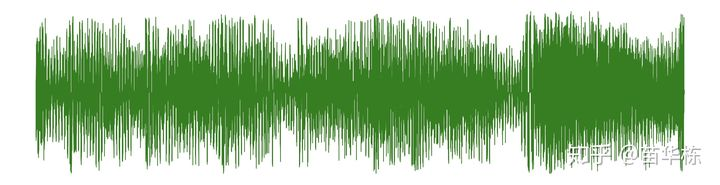
\includegraphics[width=0.6\textwidth]{figs/waveform-graph.png}
  \caption{figs:waveform-graph}
  \label{figs:waveform-graph}
\end{figure}
其中横轴是时间$t$,纵轴是振幅$A\in[-1,1]$。假设播放器读入这段音频进行音频播放,现在我想让音量大一些。由于上面波形图的振幅对应的就是声音的强度,如果想让音量大一些,只需要将整体的振幅同比例扩大即可。

  但如果我想加强这段音乐的低音部分,让音乐更厚重一些。虽然这是一段美妙的音乐,但是从时域的图像看起来,似乎杂乱无章,想找到低音部分根本无从下手,跟不用说将低音部分加强了。因为高中低音在时域中是杂糅在一起的,我们无法将他们剥离开来,随便改动波形图的一部分,都会同时影响到高中低音。所以,如果播放器仅对时域信号进行处理,是无法完成这个需求的。

  和时域的这种限制类似的还有RGB空间。任何一个颜色都可以通过R/G/B(红/绿/蓝)三原色表示出来,如图\ref{figs:rgb}。
\begin{figure}[!htb]
  \centering
  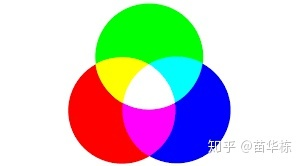
\includegraphics[width=0.6\textwidth]{figs/rgb.png}
  \caption{figs:rgb}
  \label{figs:rgb}
\end{figure}
通过调整三种颜色的配比,就能混合出各种颜色。我们经常通过RGB空间来表示所有颜色的原因在于,人类有三种视锥细胞,而这三种视锥细胞最敏感的波长接近于红/绿/蓝(如图\ref{figs:rgb-wavelength})。所以,任何颜色对于大脑来说,都是这三种视锥细胞电信号的混合作用,这也是我们使用RGB空间的生物学基础。
\begin{figure}[!htb]
  \centering
  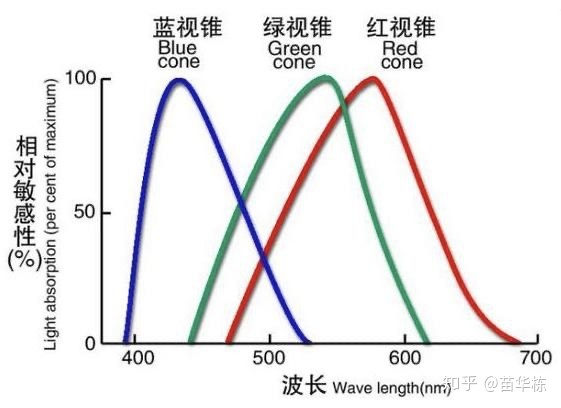
\includegraphics[width=0.8\textwidth]{figs/rgb-wavelength.png}
  \caption{figs:rgb-wavelength}
  \label{figs:rgb-wavelength}
\end{figure}

  虽然RGB空间和我们的视锥细胞原理类似,而且模型非常简单。但是在某些条件下,它仍然无法满足我们的要求。比如,我们在拍照时有时会出现红颜现象(如图\ref{figs:red-eye})。
\begin{figure}[!htb]
  \centering
  
\includegraphics[width=0.6\textwidth]{figs/red-eye.png}
  \caption{figs:red-eye}
  \label{figs:red-eye}
\end{figure}

  我们需要PS掉红眼,但是我们如何在RGB空间中找到红色的范畴呢?有人可能会说,R值越大的地方代表越红,是这样的吗?我们看(R,G,B)=(170,0,0)时,颜色如图\ref{figs:rgb-red}所示。
\begin{figure}[!htb]
  \centering
  
\includegraphics[width=0.2\textwidth]{figs/rgb-red.png}
  \caption{figs:rgb-red}
  \label{figs:rgb-red}
\end{figure}

  上图的颜色我们可以认为是红色的范围。但当(R,G,B)=(187,187,187)的时候,颜色如图\ref{figs:rgb-gray}所示。
\begin{figure}[!htb]
  \centering
  
\includegraphics[width=0.2\textwidth]{figs/rgb-gray.png}
  \caption{figs:rgb-gray}
  \label{figs:rgb-gray}
\end{figure}

  虽然R的值增大了,但是G/B值的大小也会影响混合的颜色,导致变成了灰色。所以RGB三个值,牵一发而动全身,如果想在RGB空间找到红色范围是非常困难的,这就需要将色彩从RGB空间转换到HSV空间(如图\ref{figs:hsv}),在HSV空间红色的范围可以很容易的表示出来。
\begin{figure}[!htb]
  \centering
  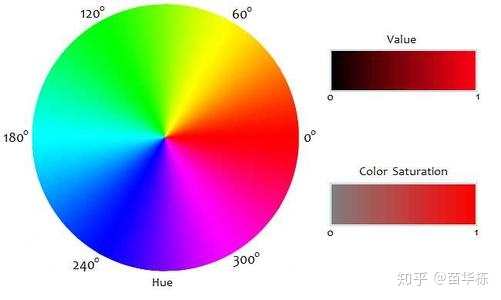
\includegraphics[width=0.6\textwidth]{figs/hsv.png}
  \caption{figs:hsv}
  \label{figs:hsv}
\end{figure}

  RGB空间就和时域一样,都有着自身的限制。所以最容易理解的表现形式并不一定是最方便计算的。我们往往需要进行一种变换,将在原来空间中难以处理的问题变换到方便计算的空间中去。

\section{频域}
  频域就是描述频率所用到的空间或者说坐标系。频率虽然比较抽象,但是在我们的生活中是无处不在的,只是我们很少直接提到这个专业名词。

  对于波来说,频率是每秒波形重复的数量。声音是一种波;光具有波粒二象性,也具有电磁波的性质;更普遍的说,频率是物质每秒钟完成周期性变化的次数。比如在家里用的交流电是50Hz,意思就是电压每秒完成50次振荡周期,如图\ref{figs:ac}所示。
\begin{figure}[!htb]
  \centering
  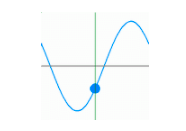
\includegraphics[width=0.2\textwidth]{figs/ac.png}
  \caption{figs:ac}
  \label{figs:ac}
\end{figure}

  而前面提到的低音效果是什么样的效果呢?就好比家庭影院中的低音炮,它是如何实现重低音的呢?简单来说,可以将它简化成一个低通滤波器,下图\ref{figs:low-pass}是低通滤波器的频率响应曲线。
\begin{figure}[!htb]
  \centering
  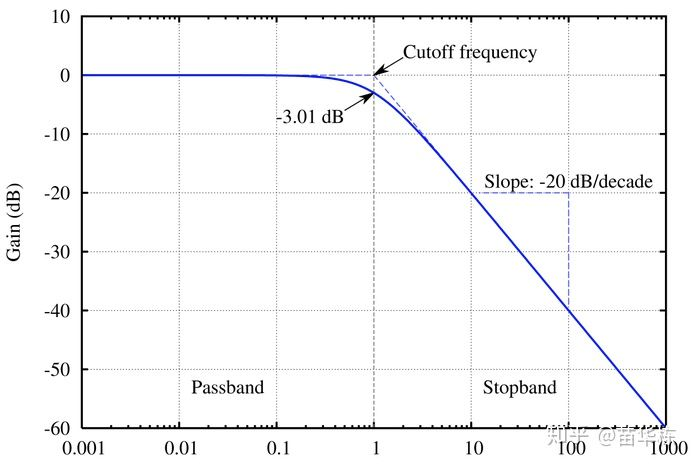
\includegraphics[width=0.6\textwidth]{figs/low-pass.png}
  \caption{figs:low-pass}
  \label{figs:low-pass}
\end{figure}
横轴是频率(Hz),纵轴是声音大小(dB)。所谓的低音效果,就是对声音中的低音部分保留或者增强,对应上图中左侧的横线部分;而对于声音中的高音部分进行衰减,对应上图中右侧的斜坡部分。通过这个低通滤波器,我们就能将低音过滤,将高音衰减。为了实现更好的视听效果,实际中,功放或播音器的实现会比这个复杂很多,上图中进行了简化。

  可见,低音效果是频率范围内考虑问题,而波形图是在时域内的图像,所以如果想在时域内解决低音效果的问题,就如同鸡同鸭讲。所以我们就要找到一个沟通时域和频域的桥梁,也就是一个翻译,让时域和频域能够无障碍的沟通。但是,时域和频域表达的又只能是同一种信息,只是表现形式不同。

  就好比人们想了解古埃及文化,但完全不了解古埃及象形文的含义,所以也就无法根据记载的文字了解当时的文化。直到商博良破译了罗塞塔石碑上的古埃及象形文,才打开了古埃及文化的大门。所谓破译,其实就是找到古埃及象形文是如何表意的,然后翻译成现有文字系统,比如希腊文。它们本质上表达的是同一种信息,只是表现形式不同。

\section{时域转频域}
\subsection{极坐标与直角坐标系类比}
  前面类比了RGB空间,解释了为什么要进行时域到频域的转换。可能还不够形象,这里再用直角坐标系和极坐标系做一个类比。我们来看一下阿基米德螺线(如下图\ref{figs:archimedes-spiral}),当一点P沿动射线OP以等速率向外运动的同时,这射线又以等角速度绕点O旋转,点P的轨迹称为“阿基米德螺线”。它的极坐标方程为:$r=a+b\theta$。这种螺线的每条臂的间距永远相等于$2{\pi}b$。
\begin{figure}[!htb]
  \centering
  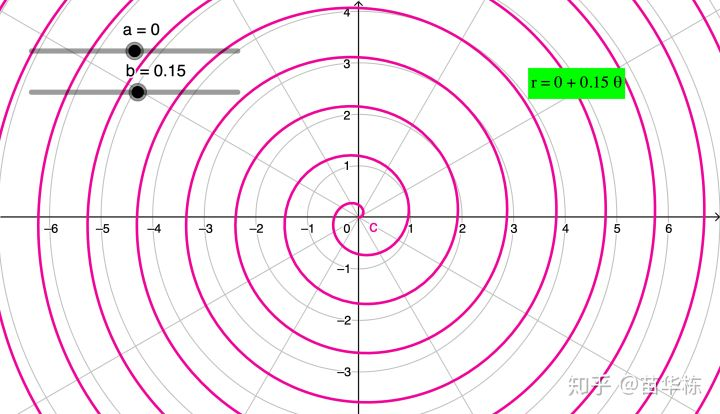
\includegraphics[width=0.6\textwidth]{figs/archimedes-spiral.png}
  \caption{figs:archimedes-spiral}
  \label{figs:archimedes-spiral}
\end{figure}

  这种曲线在极坐标系中很容易的表示出来,而且形式非常简单优雅。但是在直角坐标系下要以$X-Y$的形式表示出来确是非常困难的,只能用参数化方程来表示。也就是说,有些问题,当我们换一个空间或者说域去考虑的时候,可能会豁然开朗。
\subsection{傅里叶级数}
  为了形象的理解为什么要进行时域到频域的转换,前面已经举了很多的例子,下面正式开始进入时域和频域的变换。我们先来看一下标准正弦函数,如下图\ref{figs:sin-func}。
\begin{figure}[!htb]
  \centering
  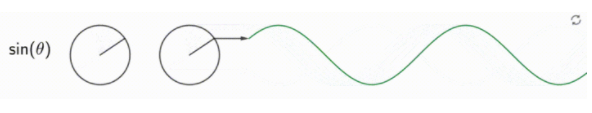
\includegraphics[width=0.8\textwidth]{figs/sin-func.png}
  \caption{figs:sin-func}
  \label{figs:sin-func}
\end{figure}
在时域它的函数方程是$y=\mathrm{sin}(x)$,而它的频率是$f=\frac{1}{T}=\frac{1}{2\pi}$。所以,上面这个函数在频域中的图像如下图\ref{figs:sin-freq}所示。
\begin{figure}[!htb]
  \centering
  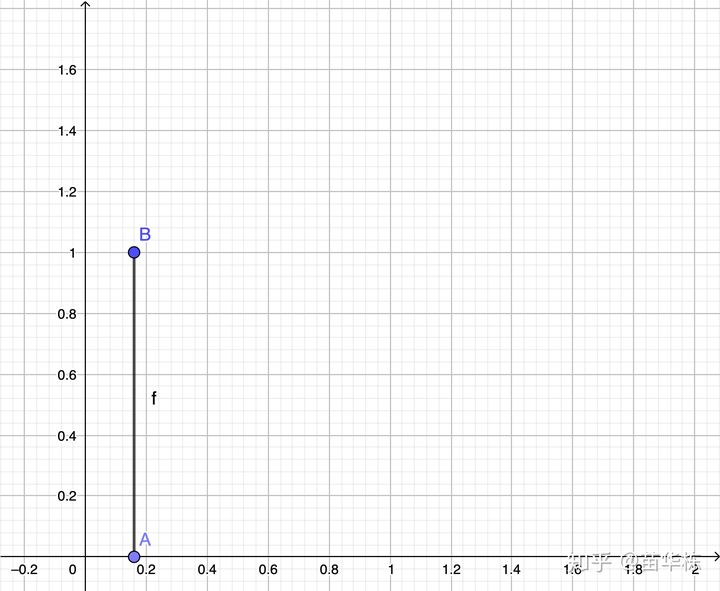
\includegraphics[width=0.6\textwidth]{figs/sin-freq.png}
  \caption{figs:sin-freq}
  \label{figs:sin-freq}
\end{figure}
横轴是频率$f$,纵轴是幅值$A$。上面两张图分别从时域和频域展示了正弦函数,但表达的都是同样的信息。

  更一般的有$y=A\mathrm{sin}(2{\pi}fx+\phi)$,其中$f$是正弦函数的频率,$\phi$是初始相位,$A$是幅度。在广义的频率中,$f$可正可负,上图中旋转臂顺时针旋转,$f$为负值。如果旋转臂转得越快,则频率越高;零时刻旋转臂和水平方向的夹角,就是初始相位。

  由于正弦函数是单一频率,在频域中只需要一根竖线就能表现出来。我们期望的也是将时域的信号转换成一个个单一频率的正弦函数的组合,这样我们就能够在频域中用一根根竖线表示出来,也就完成了从时域到频域的转换。而上面提到的正弦函数表达式可以转换成如下形式:
\begin{equation}
  \begin{aligned}
    y&=A\mathrm{sin}(2{\pi}fx+\theta)\\
     &=A\mathrm{sin}(\theta)\mathrm{cos}(2{\pi}fx)+A\mathrm{cos}(\theta)\mathrm{sin}(2{\pi}fx)\\
     &=a_{n}\mathrm{cos}(2{\pi}fx)+b_{n}\mathrm{sin}(2{\pi}fx)
  \end{aligned}
\end{equation}

  所以,如果可以将任意波形都转化成若干个正弦函数和余弦函数的线性组合,我们是不是就完成了时域到频域的转换?

  别急,实际的波形可能会有一个“直流分量”,如下图\ref{figs:rec-wave}。这个方形波并没有沿X轴往复运动,而是沿$Y=2$这条直线往复运动。对于这类的波形,单纯的用正余弦函数组合是无法表示出来的,因为正余弦都是沿X轴往复运动,所以必须叠加一个“直流分量”。
\begin{figure}[!htb]
  \centering
  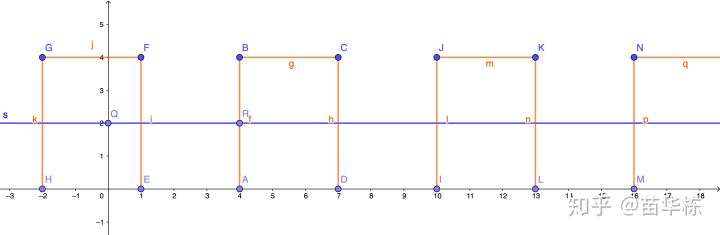
\includegraphics[width=0.6\textwidth]{figs/rec-wave.png}
  \caption{figs:rec-wave}
  \label{figs:rec-wave}
\end{figure}

  所以最后,如果任意波形都可以转化成常数、若干个正余弦函数的线性组合,我们就可以完成时域到频域的转换。用数学公式表达如下面所示:
\begin{equation}
  s_{N}(x)\overset{?}{=}\frac{a_{0}}{2}+\sum_{n=1}^{N}\left(\overbrace{a_{n}}^{A_{n}\mathrm{sin}(\phi_{n})}\mathrm{cos}(2{\pi}fnx)+\overbrace{b_{n}}^{A_{n}\mathrm{cos}(\phi_{n})}\mathrm{sin}(2{\pi}fnx)\right)
\end{equation}
上式中的$\frac{a_{0}}{2}$就对应了直流分量,我们可以把它想象成一个常数而已。于是问题就转化成,对于任意波形,我们能不能找到一组系数$a_{n}$和$b_{n}$,使上述等式成立?(为什么上式采用了离散的频率,而且都是$2{\pi}f$的整数倍呢?后面会介绍)。

  到这里,法国数学家傅里叶就必须登场了。他在1807年发表的论文中帮我们完成了这个工作,他提出了一个当时非常具有争议性的论断:任何连续周期信号都可以由一组适当的正弦曲线组合而成。

  其实,对于连续周期信号,比如上图中的周期方波,严格意义上说它的频域变换叫做傅里叶级数,因为经过频域变换后,它的频谱是离散的。而当我们现在说起傅里叶变换,默认指的是连续非周期信号的变换,如下图\ref{figs:rec-single}所示。因为非周期信号可以想象成信号的周期趋近于无穷大,所以傅里叶变换其实是对傅里叶级数的扩展。
\begin{figure}[!htb]
  \centering
  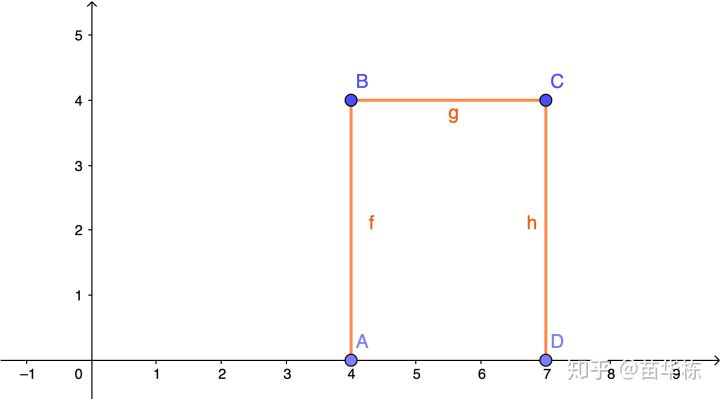
\includegraphics[width=0.6\textwidth]{figs/rec-single.png}
  \caption{figs:rec-single}
  \label{figs:rec-single}
\end{figure}

\subsection{正交性}
  我们接下来介绍的都是基于连续周期函数的频域变换,也就是傅里叶级数。重新复制一下前面要证明的等式:
\begin{equation}
  s_{N}(x)\overset{?}{=}\frac{a_{0}}{2}+\sum_{n=1}^{N}\left(\overbrace{a_{n}}^{A_{n}\mathrm{sin}(\phi_{n})}\mathrm{cos}(2{\pi}fnx)+\overbrace{b_{n}}^{A_{n}\mathrm{cos}(\phi_{n})}\mathrm{sin}(2{\pi}fnx)\right)
\end{equation}
在我们尝试求解系数$a_{n}$和$b_{n}$之前,我们先解释一下前面留下的问题。上式为什么采用了离散的频率,而且都是$2{\pi}f$的整数倍呢?

  这样的一组正余弦函数除了可以表示单一频率之外,方便的在频域表示,而且组成一组正交基,具有两两正交的优质特性,可以方便的计算系数。

  我们知道,正交是线性代数里的概念,是垂直这一直观概念的推广。比如,在欧几里得空间中,正交就是两个向量的内积为零。如下式:
\begin{equation}
  \left\langle(x_{1},\cdot\cdot\cdot,x_{n}),(y_{1},\cdot\cdot\cdot,y_{n})\right\rangle=\sum_{i=1}^{n}x_{i}y_{i}=x_{1}y_{1}+\cdot\cdot\cdot+x_{n}y_{n}=0
\end{equation}
  下图\ref{figs:axis-xyz}中,X、Y、Z三个轴就是两两正交的。因为X、Y、Z三个轴对应的向量分别是(1,0,0),(0,1,0),(0,0,1),根据上面的内积公式可得他们两两内积为零。
\begin{figure}[!htb]
  \centering
  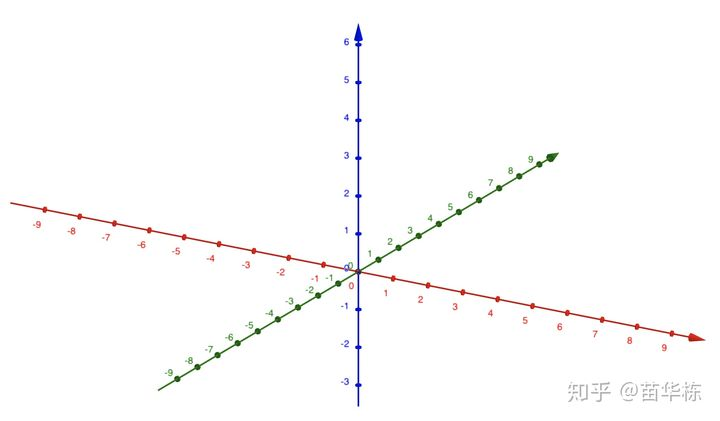
\includegraphics[width=0.6\textwidth]{figs/axis-xyz.png}
  \caption{figs:axis-xyz}
  \label{figs:axis-xyz}
\end{figure}

  那对于两个连续函数来说,应该如何表示正交呢?函数在某个区间内部有无穷多个点,无法直接套用内积公式。但我们可以借鉴积分的思想,将函数在一段连续区间分割成一份一份,这样每一份的取值合起来就可以组成一个向量,于是可以用向量的内积来表示两个函数是否正交,如下图\ref{figs:func-seg}所示。
\begin{figure}[!htb]
  \centering
  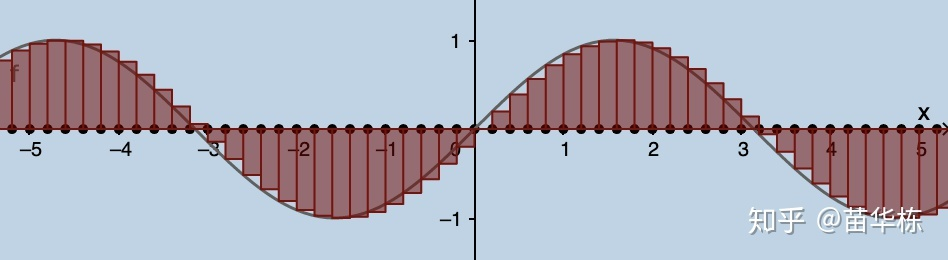
\includegraphics[width=0.6\textwidth]{figs/func-seg.png}
  \caption{figs:func-seg}
  \label{figs:func-seg}
\end{figure}
当分割的区间无限小时,向量变成无限维,于是向量的内积就可以用积分来替代了。所以两个函数的正交其实可以用积分来表示。
\begin{figure}[!htb]
  \centering
  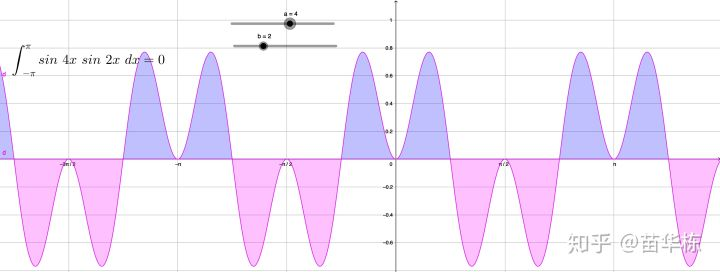
\includegraphics[width=0.6\textwidth]{figs/func-seg-4x2x.png}
  \caption{figs:func-seg-4x2x}
  \label{figs:func-seg-4x2x}
\end{figure}
对于$\mathrm{sin}4x$和$\mathrm{sin}2x$,在一个周期内,处于X轴上方的面积和X轴下方的面积相等,所以这两个函数的积分为0,也就是互相正交的。还有另外一种情况
\begin{figure}[!htb]
  \centering
  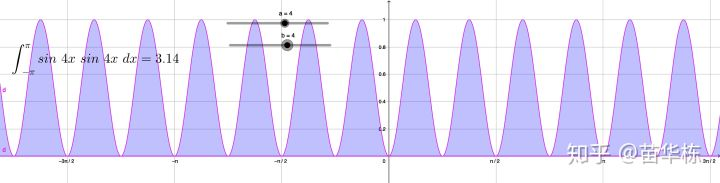
\includegraphics[width=0.6\textwidth]{figs/func-seg-4x4x.png}
  \caption{figs:func-seg-4x4x}
  \label{figs:func-seg-4x4x}
\end{figure}
积分的两个函数相同,都是$\mathrm{sin}4x$,这时积分结果都在X轴上方,积分大于0,也就是不相互正交。

  更一般的情况,有
\begin{equation}
  \begin{aligned}
    &\begin{cases}
      \int_{-\pi}{\pi}\mathrm{cos}(mx)\mathrm{cos}(nx)dx=\pi, m=n,m,n{\geq}1\\
      \int_{-\pi}{\pi}\mathrm{cos}(mx)\mathrm{cos}(nx)dx=0, m{\neq}n,m,n{\geq}1
    \end{cases}\\
    &\begin{cases}
      \int_{-\pi}{\pi}\mathrm{sin}(mx)\mathrm{sin}(nx)dx=\pi, m=n,m,n{\geq}1\\
      \int_{-\pi}{\pi}\mathrm{sin}(mx)\mathrm{sin}(nx)dx=0, m{\neq}n,m,n{\geq}1
    \end{cases}\\
    &\int_{-\pi}{\pi}\mathrm{cos}(mx)\mathrm{sin}(nx)dx=0, m,n{\geq}1\\
    &\int_{-\pi}{\pi}\mathrm{cos}(nx)dx=0, n{\geq}1\\
    &\int_{-\pi}{\pi}\mathrm{sin}(nx)dx=0, n{\geq}1
  \end{aligned}
\end{equation}
所以,1、$\mathrm{cos}(x)$、$\mathrm{sin}(x)$、$\mathrm{cos}(2x)$、$\mathrm{sin}(2x)$、$\cdot\cdot\cdot$、$\mathrm{cos}(nx)$、$\mathrm{sin}(nx)$不仅能够表示单一频率,而且还构成了一组正交基。于是我们重新看上面要证明的等式,如下所示:
\begin{equation}
  s_{N}(x)\overset{?}{=}\frac{a_{0}}{2}+\sum_{n=1}^{N}\left(\overbrace{a_{n}}^{A_{n}\mathrm{sin}(\phi_{n})}\mathrm{cos}(2{\pi}fnx)+\overbrace{b_{n}}^{A_{n}\mathrm{cos}(\phi_{n})}\mathrm{sin}(2{\pi}fnx)\right)
\end{equation}
上面这个等式和前面提到的正交基不同的仅仅是频率$2{\pi}f$,当积分区间修改成对应的周期范围内,则所有的特性完全一样。

  也就是说如果上面这个等式能成立,将是一个非常完美的等式。我们不仅完美的将它转换成了频域,用单一频率的正余弦函数组合表示出来,而且他们还是一组正交基,从线性代数的角度来看就是线性无关的,彼此互不影响,就和欧几里得空间中的X-Y-Z轴一样,无论我如何修改X的值,对Y和Z都是没有任何影响的。

  这种正交的特性可以让我们非常方便的求出对应的系数。比如我想求出$a_{10}$,它的系数就是$\mathrm{cos}(2{\pi}f{\times}10{\times}x)$,前面已经提到,$\mathrm{cos}(2{\pi}f{\times}10{\times}x)$是正交基中的一个基底,它只与自身积分不等于零,而与正交基中任意其它基底积分都为0。

  有了这个非常好的特性以后,我们要求$a_{n}$,只需在两边同时乘以$\mathrm{cos}(2{\pi}f{\times}10{\times}x)$,然后做积分,其它所有的频率部分因为正交性,都变为零,等号右侧只保留了$a_{n}$的部分,我们可以求出$a_{10}$。

  更一般地,对于$a_{n}$和$b_{n}$,有如下等式成立
\begin{equation}
  \begin{aligned}
    &a_{n}=2f\int_{x_{0}}^{x_{0}+\frac{1}{f}}s(x){\cdot}\mathrm{cos}(2{\pi}fnx)dx\\
    &b_{n}=2f\int_{x_{0}}^{x_{0}+\frac{1}{f}}s(x){\cdot}\mathrm{sin}(2{\pi}fnx)dx
  \end{aligned}
\end{equation}
到这里,我们利用正交性求出了傅里叶级数中的$a_{n}$和$b_{n}$,求解过程中没有那么严谨,只是能够直观地理解如何进行时域到频域的转换,以及如何利用正交的特性去求解系数。

\subsection{过冲现象}
  虽然求解出来了,但是真的如傅里叶所说,我们可以用正弦波去表示任意的连续周期函数吗?以方波为例,我们看下图\ref{figs:overshoot}。
\begin{figure}[!htb]
  \centering
  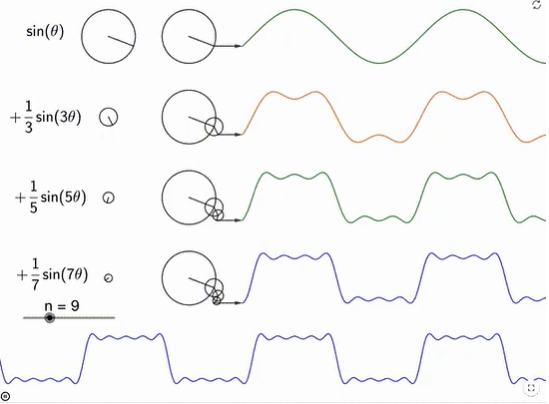
\includegraphics[width=0.6\textwidth]{figs/overshoot.png}
  \caption{figs:overshoot}
  \label{figs:overshoot}
\end{figure}
如上图,随着频率越来越丰富,合成的波形也越来越接近方波了,当$n$趋近于无穷大,也就是频谱范围无限大的时候,就可以无限逼近方波了。

  但是,我们注意到,即便在$n=29$的时候,合成的方波还是棱角处还是有一定的过冲。而且我们发现,在n增大到29的过程中,这个过冲并没有明显的减小。那么在n趋近于无穷的时候真的能够避免这种过冲吗?

  我们知道,正弦函数是一个处处连续且可导的函数,也就是说正弦函数是一个比较圆润的函数;而方波却是有棱角的,在棱角处是不连续的。一个圆润的函数最后可以合成一个带有棱角的函数吗?即使将频谱范围扩展到无穷大,就真的能够逼近出棱角吗?

  事实上,当初拉格朗日也是拿这一点反驳傅里叶的。在不连续点的过冲即使频域扩展到无穷,过冲也不会降为零的。其实傅里叶所说的逼近其实是能量的无限逼近,也就是经过傅里叶变换后的波形能量和原始波形能量可以无限逼近。

\section{复频域傅里叶级数}
  到此,基于三角函数形式的傅里叶变换已经介绍完毕。但傅里叶变换还有一种复频域的表示方式,通过复频域表示更加简单直观,但这就需要用到大名鼎鼎的欧拉公式:
\begin{equation}
  e^{ix}=\mathrm{cos}x+i\mathrm{sin}x, {\forall}x{\in}\mathbb{R}
\end{equation}

  通过复频域表示时,会出现虚数单位,而这个是我们在三角级数表现方式中不曾出现的,而最后复频域表示方式要能够化成和三角级数的相等的表达形式,所以必须想办法消掉虚数单位。所以我们就想到共轭复数$e^{-ix}=\mathrm{cos}x+i\mathrm{sin}x$。有了共轭复数,我们可以通过两个互为共轭的复数加法将虚数消掉。于是有下面的式子,我们将频域的$[1,N]$求和和常数转化成复频域的$[-N,+N]$求和,这样通过构造$-N$,就会出现两个互为共轭的复数。
\begin{equation}
  \begin{aligned}
    s_{N}(x)&\overset{?}{=}\frac{a_{0}}{2}+\sum_{n=1}^{N}\left(\overbrace{a_{n}}^{A_{n}\mathrm{sin}(\phi_{n})}\mathrm{cos}(2{\pi}fnx)+\overbrace{b_{n}}^{A_{n}\mathrm{cos}(\phi_{n})}\mathrm{sin}(2{\pi}fnx)\right)\\
      &=\sum_{n=-N}^{N}c_{n}{\cdot}e^{i2{\pi}fnx}\\
      &=\sum_{n=-N}^{N}c_{n}{\cdot}(\mathrm{cos}(2{\pi}fnx)+i\mathrm{sin}(2{\pi}fnx))
  \end{aligned}
\end{equation}
然后,我们用待定系数的方式求解$c_{n}$:
\begin{equation}
  c_{n}=\begin{cases}
    p+iq,(n \ge 0)\\
    p-iq,(n \le 0)
  \end{cases}
\end{equation}
将互为共轭的两个系数提取出来,对比三角级数和复频域的表示方式,列出等式:
\begin{equation}
  \begin{aligned}
    &(p-iq)(\mathrm{cos}(2{\pi}fnx)-i\mathrm{sin}(2{\pi}fnx))+(p+iq)(\mathrm{cos}(2{\pi}fnx)+\mathrm{sin}(2{\pi}fnx))\\
    =&a_{n}\mathrm{cos}(2{\pi}fnx)+b_{n}\mathrm{sin}(2{\pi}fnx))
  \end{aligned}
\end{equation}
解得$p=\frac{a_{n}}{2}$,$q=-\frac{b_{n}}{2}$,于是有如下表达式:
\begin{equation}
  c_{n}\overset{def}{=}\begin{cases}
    \frac{1}{2}(a_{n}-ib_{n}),n{\ge}0\\
    \frac{1}{2}a_{0},n=0\\
    c_{\left|n\right|}^{*},n{\le}0
  \end{cases}
\end{equation}
所以,我们有了复频域的傅里叶级数表示方式。如果想要求出$c_{n}$,同三角级数一样,在复频域上$e^{i2{\pi}fnx}$同样具有正交性,所以我们想要求出$c_{n}$,只需要在等式两边同时乘以$e^{-i2{\pi}fnx}$,然后再进行积分们就可以过滤掉其它复频率分量,而只保留$c_{n}$,于是我们有
\begin{equation}
  c_{n}=f\int_{x_{0}}^{x_{0}+\frac{1}{f}}s(x){\cdot}e^{-i2{\pi}fnx}dx
\end{equation}

\section{结尾}
  傅里叶就是在它的《热的解析理论》中提出了傅里叶变换的一系列思想,虽然他如此伟大,但是他最后的结局却是“no zuo no die”排行榜第一。

  傅里叶对热极为痴迷,同时认为热是世界上的最棒的东西,甚至可以包治百病!他为了证明这个理论,一次他在身体不舒服的时候,在大热天,他把门窗四闭,烤着火炉,“治疗”着自己。变态的室温大大加重了他的病情,最终活活自己热死了。。。

  1830年5月16日,傅里叶卒于法国巴黎。

\section{欣赏}
  到此,我们已经介绍完了傅里叶级数的三角函数和复频域形式。最后,我们欣赏一下傅里叶变换都能够模拟什么样的波形。
\begin{figure}[!htb]
  \centering
  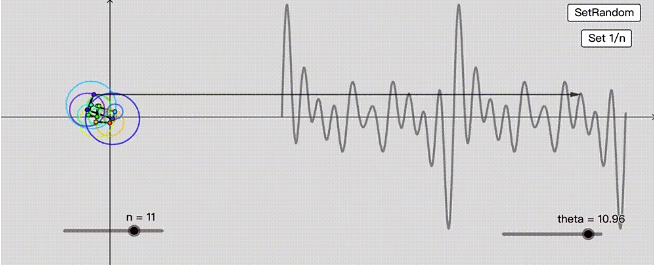
\includegraphics[width=0.6\textwidth]{figs/electrocardiogram.png}
  \caption{figs:electrocardiogram}
  \label{figs:electrocardiogram}
\end{figure}

  如果你觉得傅里叶级数只能画上面的“心电图”,那你太小看它了,我甚至可以用它来画恐龙,下面这张图是由50个频率的傅里叶级数组成,在我本地跑了将近4分钟(实在太卡),20倍速播放。
\begin{figure}[!htb]
  \centering
  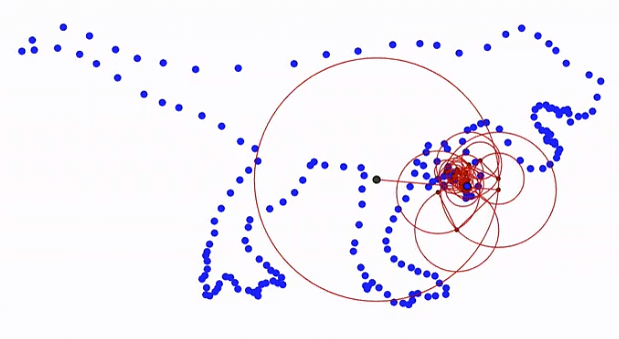
\includegraphics[width=0.6\textwidth]{figs/dinosaur.png}
  \caption{figs:dinosaur}
  \label{figs:dinosaur}
\end{figure}

  画一只可爱的小猫也不是不可以~
\begin{figure}[!htb]
  \centering
  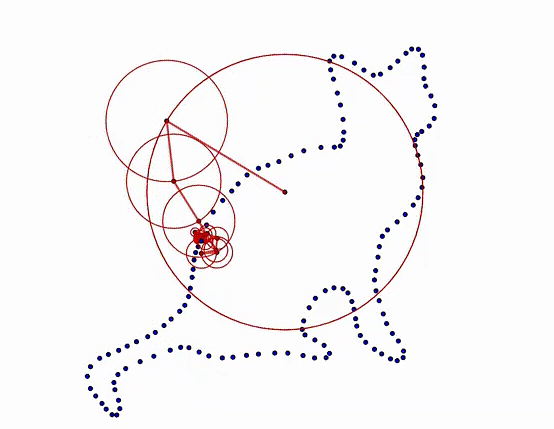
\includegraphics[width=0.6\textwidth]{figs/cat.png}
  \caption{figs:cat}
  \label{figs:cat}
\end{figure}

  傅里叶发现了这么伟大的公式,连接了频域和时域,其实给我们带来的更多的是思维上的转变。当我们在时间轴上思考问题比较困难时,是不是可以换一个维度重新审视思考或许会豁然开朗。

\nocite{*}
\bibliography{ref/refs}

\end{document}
